\documentclass{article}
\usepackage{graphics, amsmath, amssymb, multirow}
\usepackage{geometry} 
\geometry{
  a4paper,
  total={170mm,257mm},
  left=20mm,
  top=20mm,
}

\begin{document}

\section{Image Tests}

Inline image: 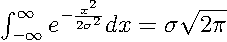
\includegraphics[width=0.15\textwidth]{test.png}

\begin{figure}[h]
    \centering
    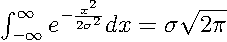
\includegraphics[width=0.7\textwidth]{test.png}
    \caption{Test image centered in a figure environment.}
    \label{fig:test_image}
\end{figure}

\newpage

\section{Some beautiful mathematical equations}

Ramanujan's formula:

$$\frac{1}{\pi}=\frac{2\sqrt{2}}{9801}\sum_{k=0}^\infty\frac{(4k)! (1103+26390k)}{(k!)^4 396^{4k}}$$

Euler's formula: $e^{i\pi}+1=0$

Area of triangle with sides a,b,c is: 

$$A=\frac{1}{2} \sqrt{s(s-a)(s-b)(s-c)},\quad s=\frac{a+b+c}{2}$$

The most important formula in calculus:

\[
  f'(x)=\lim_{h\to 0}\frac{f(x+h)-f(x)}{h}
\]

Einstain's field equations:

\[
R_{\mu\nu}-\frac{1}{2}g_{\mu\nu}R+\Lambda g_{\mu\nu}=\frac{8\pi G}{c^4}T_{\mu\nu}
\]

Gamma function:

\[
  \Gamma(z) = \int_0^\infty t^{z-1} e^{-t} dt,\quad\Gamma(z+1) = z \Gamma(z)
\]

Pythagora's theorem:

$$a^2+b^2=c^2$$

Logarithms: 

$$\log ab=\log a+\log b$$

Navier-Stokes equation:

$$\rho\left(\frac{\partial \textbf{v}}{\partial t}+\textbf{v}\cdot\nabla\textbf{v}\right)+\nabla p-\nabla\cdot\textbf{T}=\textbf{f}$$

Law of gravity:

$$F=G\frac{m_1m_2}{r^2}$$

Fourier transform:

\[
  F(\omega) = \int_{-\infty}^\infty f(t) e^{-2\pi i t \omega} dt
\]

Maxwell's equations: 

\begin{equation}
\nabla \times \textbf{E}=\frac{\rho}{\epsilon_0}
\end{equation}

\begin{equation*}
\nabla \cdot \textbf{H}=0
\end{equation*}

\begin{equation*}
\nabla \times \textbf{E}=-\frac 1c\frac{\partial \textbf{H}}{\partial t}
\end{equation*}

\begin{equation*}
\nabla \times \textbf{H}=\frac 1c\frac{\partial \textbf{E}}{\partial t}
\end{equation*}

Schroedinger equation:

\[
i \hbar \frac{\partial \psi}{\partial t} = H\Psi
\]

Chaos theory:

$$x_{t+1}=kx_t(1-x_t)$$

Information theory:

\[
  H=-\sum p(x)\log p(x)
\]

Black-Scholes equation:

$$\frac12\sigma^2S^2\frac{\partial^2V}{\partial S^2}+rS\frac{\partial V}{\partial S}+\frac{\partial V}{\partial t}-rV=0$$

Second law or thermodynamics:

$$dS\ge 0$$

Mass-energy equivalence:

$$E=mc^2$$

Basel problem:
\[
  \frac{\pi^2}{6}=\sum_{n=1}^\infty \frac{1}{n^2}
\]

Euler-Mascheroni constant:

\[
\gamma = \lim_{n\to\infty}(\sum_{n=1}^\infty \frac{1}{n}-\log n)=\int_1^\infty\left(-\frac1x+\frac1{\lfloor x\rfloor}\right)\,\mathrm dx\approx 0.5772156649015328606065120\ldots
\]

Binomial expansion:

\[
(a+b)^n = \sum_{k=0}^n \binom{n}{k} a^k b^{n-k}  
\]

Gauss:

$$\int_{-\infty}^\infty e^{-x^2} dx = \sqrt{\pi}$$

The Callan-Symanzik equation:

\[
\left[M\frac{\partial}{\partial M}+\beta(g)\frac{\partial}{\partial g}+n\gamma\right]G^n(x_1,x_2,...,x_n;M,g)=0
\]

Minimal surface equation:

$$\mathcal{A}(u)=\int_\Omega(1+|\nabla u|^2)^{1/2} dx_1 dx_2 ... dx_n$$ 

Multiline equations:

\begin{eqnarray*}
\cos{2\theta} & = & \cos^2\theta - \sin^2\theta \\
              & = & 2\cos^2\theta - 1 \\
              & = & 1 - 2\sin^2\theta
\end{eqnarray*}

And finally:

$$1=0.999999999999999999\ldots$$

Just for fun: $6 + 9 + 6 \cdot 9 = 69$

Quadratic equation:

\[
  ax^2+bx+c=0 \implies x_{1,2}=\frac{-b\pm\sqrt{b^2-4ac}}{2a}  
\]

Four more ways to calculate pi:

\begin{equation*}
  \pi=\sum_{k=0}^\infty\left[\frac{1}{16^k}\left(\frac{4}{8k+1}-\frac{2}{8k+4}-\frac{1}{8k+5}-\frac{1}{8k+6} \right) \right]
\end{equation*}

\begin{equation*}
  \frac{2}{\pi}=\frac{\sqrt{2}}{2}\cdot\frac{\sqrt{2+\sqrt{2}}}{2}\cdot\frac{\sqrt{2+\sqrt{2+\sqrt{2}}}}{2}\cdot\ldots
\end{equation*}

\begin{equation*}
\pi = 3+\textstyle \cfrac{1}{7+\textstyle \cfrac{1}{15+\textstyle \cfrac{1}{1+\textstyle \cfrac{1}{292+\textstyle \cfrac{1}{1+\textstyle \cfrac{1}{1+\textstyle \cfrac{1}{1+\ddots}}}}}}}
\end{equation*}

Chudnovsky Formula:

\[
\frac{1}{\pi} = \frac{\sqrt{10005}}{4270934400} \sum_{k=0}^\infty \frac{(6k)! (13591409 + 545140134k)}{(3k)!\,k!^3 (-640320)^{3k}}
\]

Cauchy's integral formula:

$$f(a)=\frac{1}{2\pi i}\int_{C} \frac{f(z)}{z-a} dz $$

Stirling's factorial approximation:
$$n! = \sqrt{2 \pi n} \left( \frac{n}{e} \right)^n \left( 1 + O \left( \frac{1}{n} \right) \right)$$

Taylor's series:

$$f(x)=\sum_{n=0}^\infty \frac{f^{(n)}(a)}{n!} (x-a)^n$$

Graham's number, the biggest number ever used in a scientific paper:

\[
\left.
 \begin{matrix}
  G &=&3\underbrace{\uparrow \uparrow \cdots \cdots \cdots \cdots \cdots \uparrow}3 \\
    & &3\underbrace{\uparrow \uparrow \cdots \cdots \cdots \cdots \uparrow}3 \\
    & & \underbrace{\qquad \quad \vdots \qquad \quad} \\
    & &3\underbrace{\uparrow \uparrow \cdots \cdots \uparrow}3 \\
    & &3\uparrow \uparrow \uparrow \uparrow3
 \end{matrix}
\right \} \text{64 layers}
\]

Prime number approximation:

$$ n \left( \log n + \log \log n - 1 + \frac{\log \log n - 2.1}{\log n} \right) \le p_n \le n \left( \log n + \log \log n - 1 + \frac{\log \log n - 2}{\log n} \right)$$

Prime counting function approximation:

\[
\frac{x}{\log x} \left( 1 + \frac{1}{\log x} + \frac{2}{\log^2 x} \right) \le \pi(x) \le \frac{x}{\log x} \left( 1 + \frac{1}{\log x} + \frac{2}{\log^2 x} + \frac{7.59}{\log^3 x} \right)
\]

Riemann's zeta function (automatically scaled to fit the allowed width):

\[
\zeta(s) = \sum_{n=1}^\infty \frac{1}{n^s} = \frac{1}{\Gamma(s)} \int_0^\infty \frac{x ^ {s-1}}{e ^ x - 1} \, \mathrm{d}x = \prod_{p \text{ prime}} \frac{1}{1-p^{-s}} = \frac{1}{1-2^{-s}}\cdot\frac{1}{1-3^{-s}}\cdot\frac{1}{1-5^{-s}}\cdot\frac{1}{1-7^{-s}}\cdot\frac{1}{1-11^{-s}} \cdots \frac{1}{1-p^{-s}} \cdots
\]

The most famous unsolved mathematical problem (Riemann's hypothesis):

\[
  \zeta(s) = \sum_{n=1}^\infty \frac{1}{n^s} = 0\ \land \ \mathrm{Re}(s) > 0 \implies \mathrm{Re}(s)=\frac12
\]

\end{document}


